\section{Tools} \label{sec:tools}

This section of the paper describes the tools used for the scrub process. With the requirement for agility, collaborative working and ease of linking to existing tools, Google Workspace  is the chosen platform onto which the scrub tools have been developed. The tool, called the Scrub Sandbox,  needs to facilitate the following:

\begin{enumerate}
\item Capturing the current state.
\item Capturing what the desired change is.
\item Inputting flow down milestones for the upcoming FY based on higher level milestones defined by the directors office.
\item Standardize inputs coming in from the department and teams.
\item Easily seeing the impact of the desired change on labor and non-labor budget.
\end{enumerate}

\begin{figure}[h!]
\begin{centering}
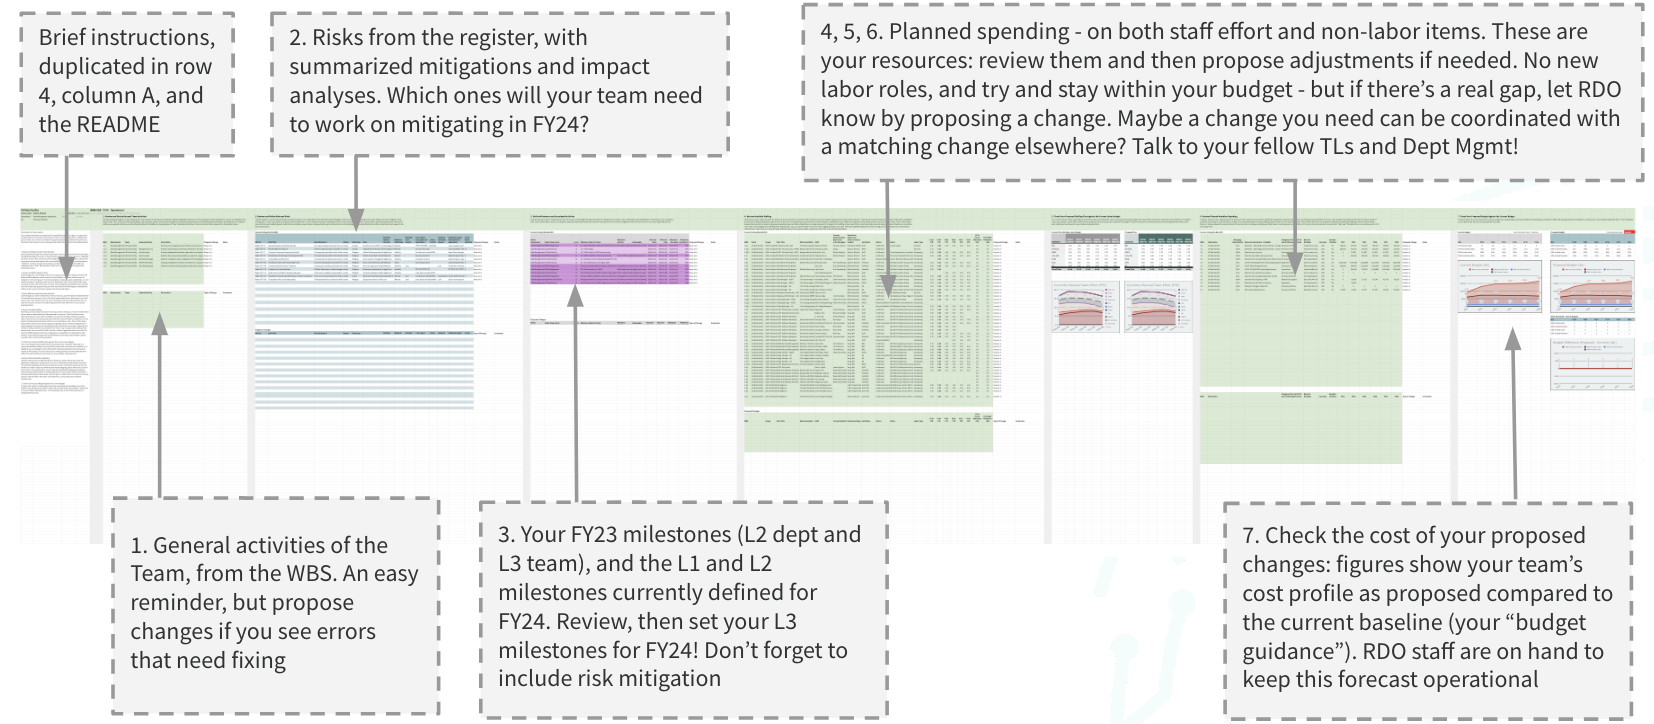
\includegraphics[width=1.0\textwidth]{Figure3OverviewScrubSandbox}
	\caption{ Overview of Scrub Sandbox
\label{fig:sandbox}}
\end{centering}
\end{figure}

\noindent Furthermore, the tool needs to enable the following areas to be scrubbed:
\begin{enumerate}
\item Work Breakdown Structure (WBS).
\item Risks.
\item Milestones.
\item Labor expenditure.
\item Non-labor expenditure.
\end{enumerate}

In all the above cases, a standard approach is applied to propose changes See \autoref{fig:wbs}. The Proposed Change column is where any needed changes are flagged. During the scrub review, a value is chosen from the drop down choices which are Keep As-Is, Modify, Remove/Replace. There is space to enter a note if explanation is needed.
If either the value Modify or Addition is chosen it will require a corresponding entry in the Proposed Changes table.
Proposed changes to the labor and non-labor plan are visualized in monetary terms in real-time with baseline comparison charts such as those shown in \autoref{fig:baseline}.



\begin{figure}[h!]
\begin{centering}
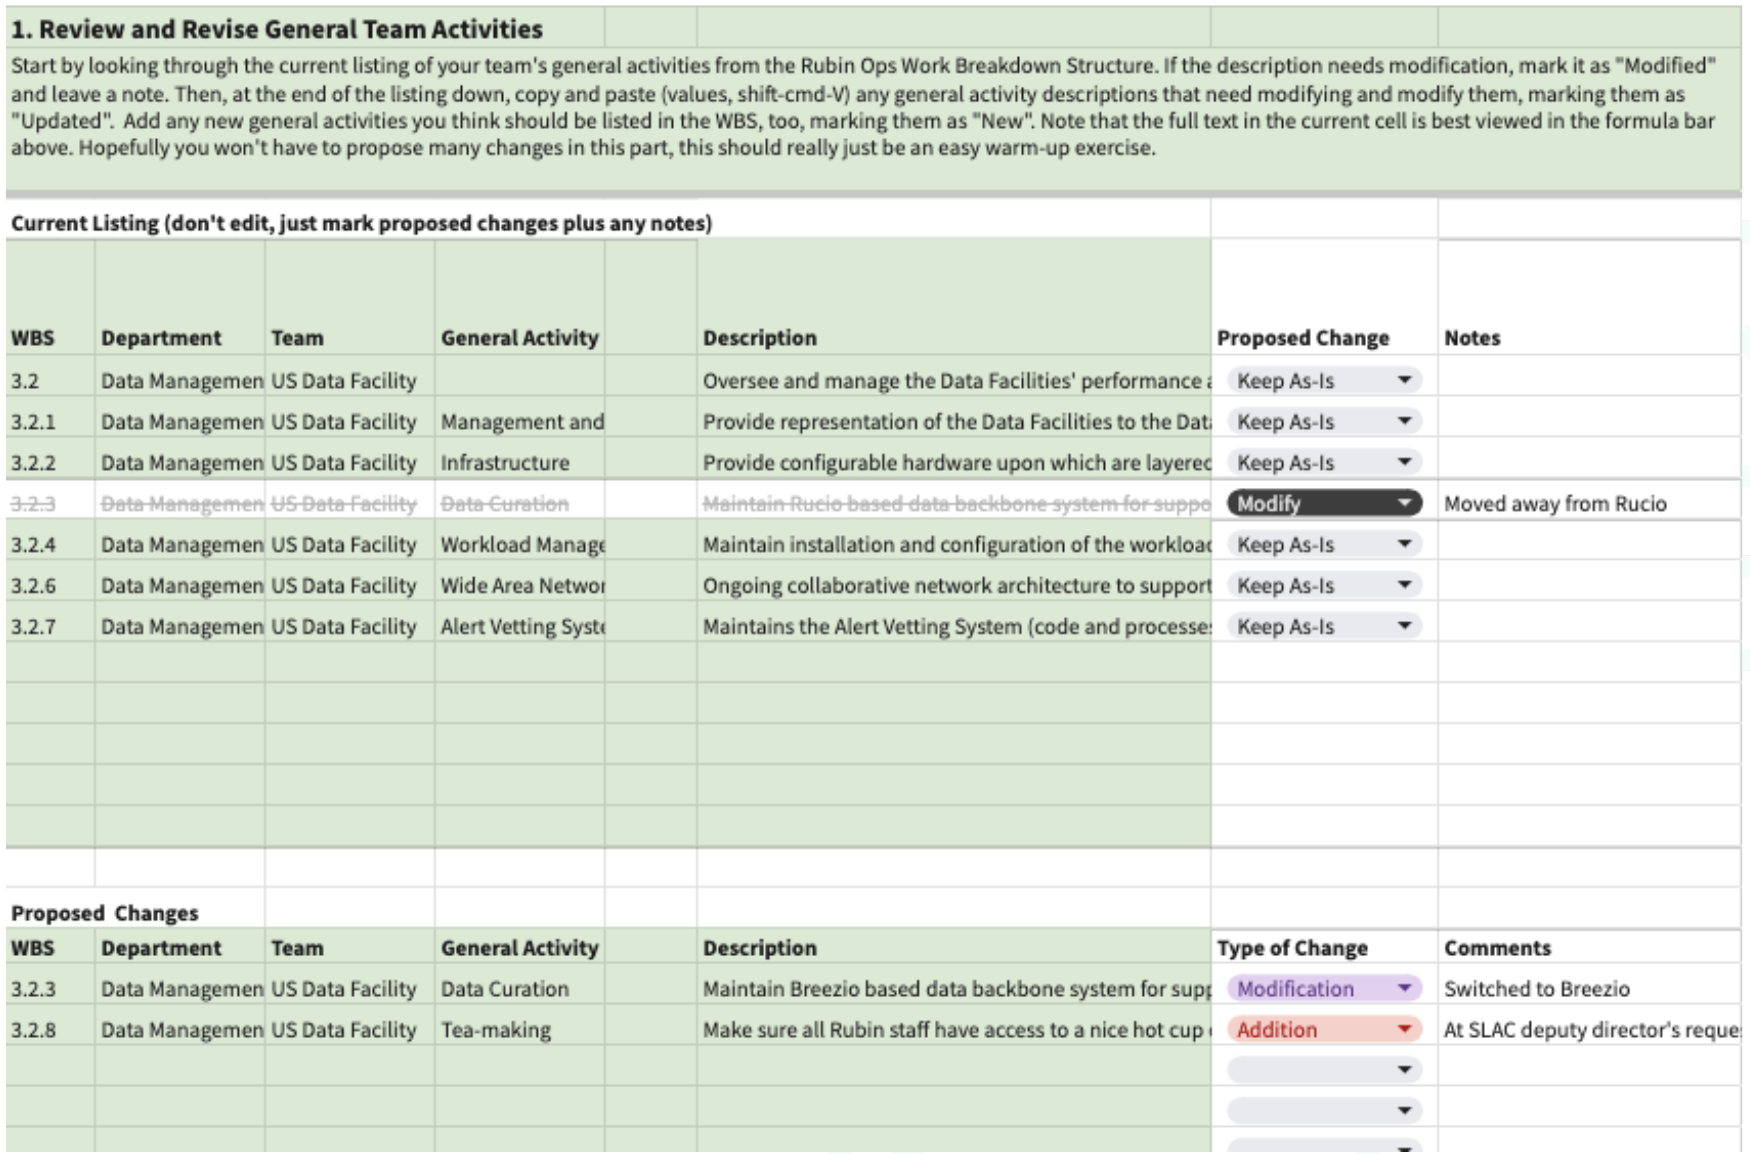
\includegraphics[width=1.0\textwidth]{Figure4WorkBreakdownStructurescrubbing}
	\caption{ Work Breakdown Structure scrubbing
\label{fig:wbs}}
\end{centering}
\end{figure}

\begin{figure}[hb!]
\begin{centering}
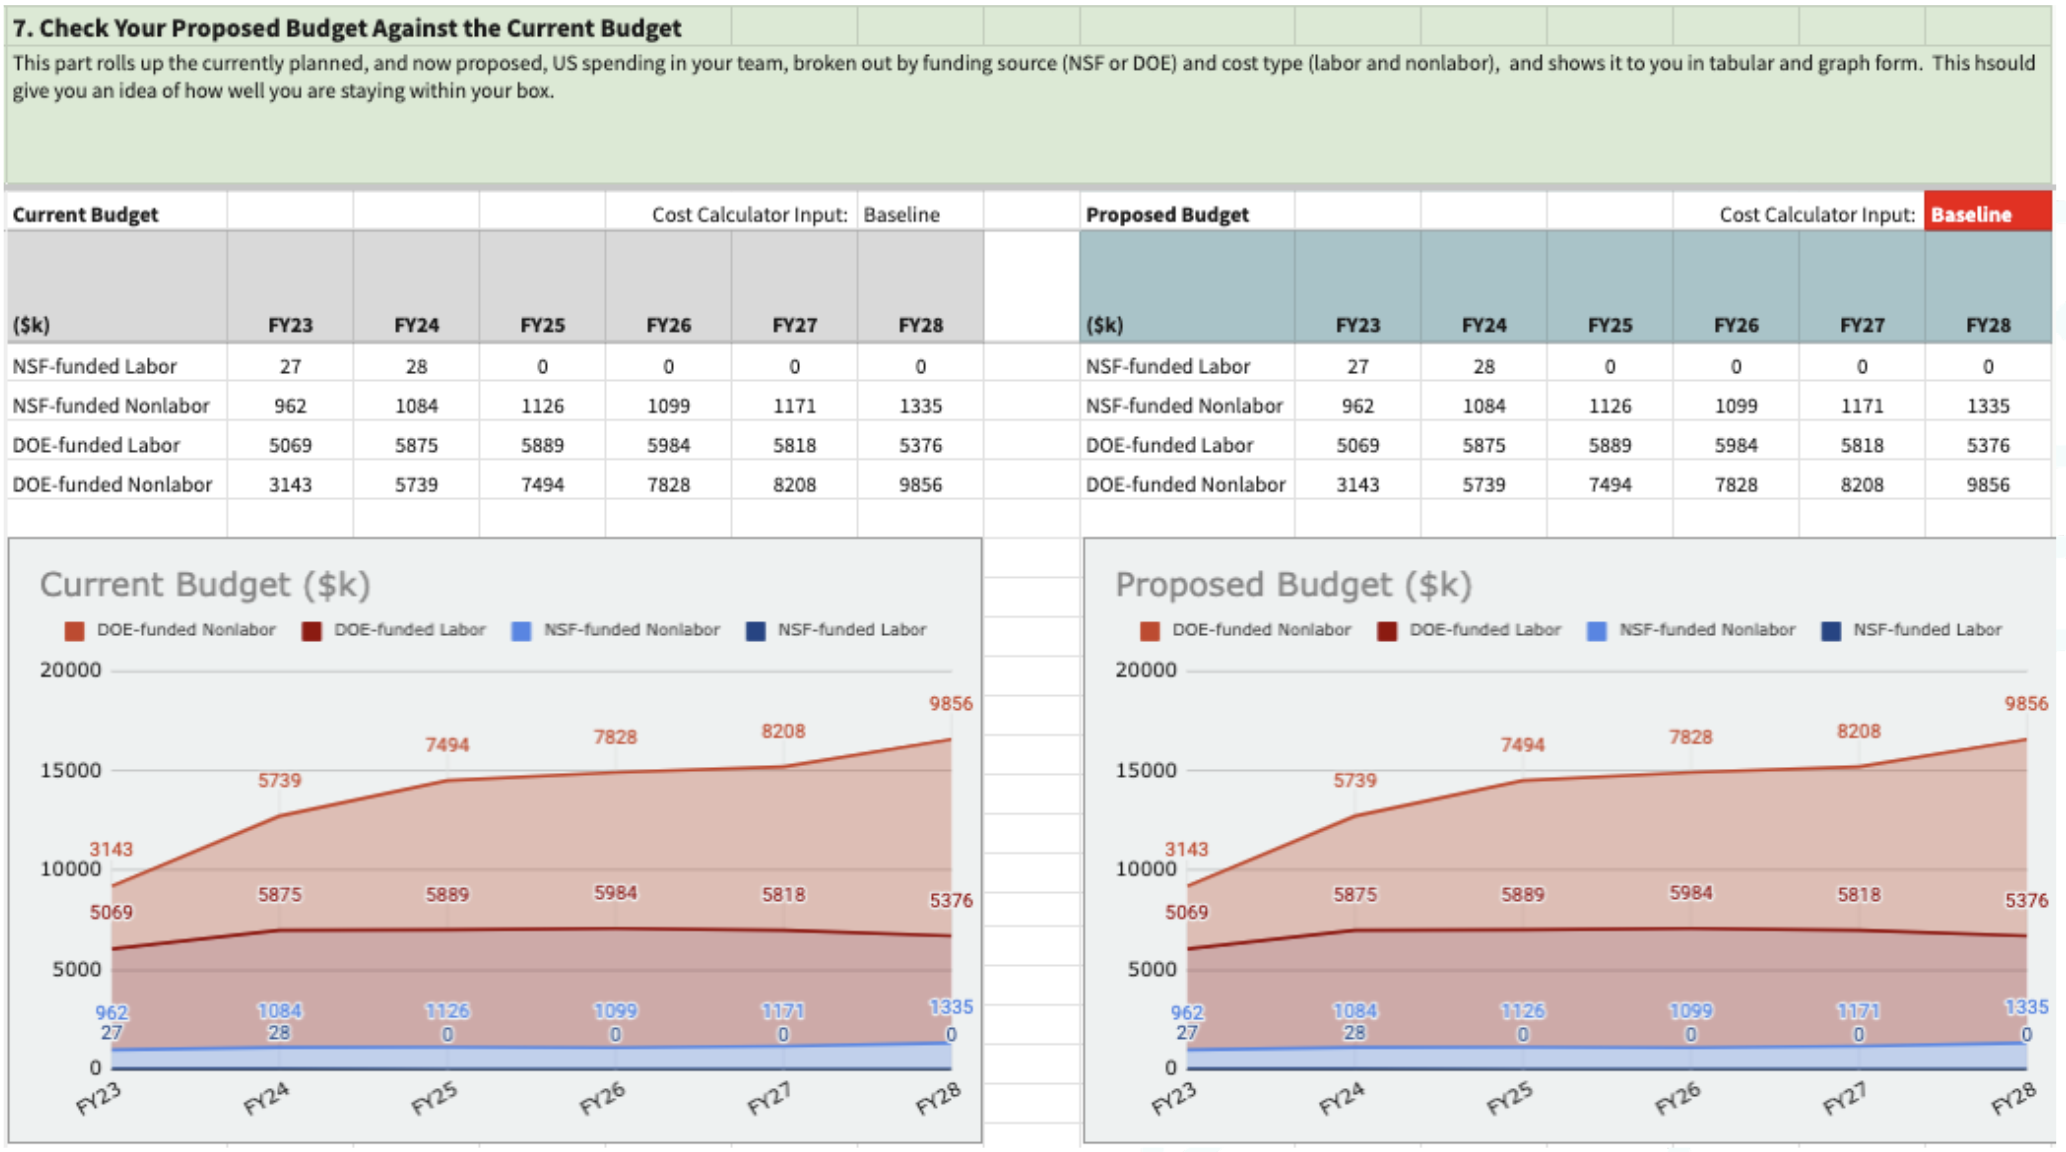
\includegraphics[width=1.0\textwidth]{Figure5BaselinevsProposed}
	\caption{Baseline vs Proposed labor and non-labor comparison
\label{fig:baseline}}
\end{centering}
\end{figure}
